\documentclass[12pt]{article}
 
\usepackage[margin=1in]{geometry}
\usepackage{amsmath,amsthm,amssymb, mathtools}
\usepackage[T1]{fontenc}
\usepackage{lmodern}
\usepackage{fixltx2e}
\usepackage[shortlabels]{enumitem}
\usepackage{tikz}
\usepackage{pgfplots}
\usepackage{float}
 
\newcommand{\N}{\mathbb{N}}
\newcommand{\R}{\mathbb{R}}
\newcommand{\Z}{\mathbb{Z}}
\newcommand{\Q}{\mathbb{Q}}
 
\newenvironment{theorem}[2][Theorem]{\begin{trivlist}
\item[\hskip \labelsep {\bfseries #1}\hskip \labelsep {\bfseries #2.}]}{\end{trivlist}}
\newenvironment{lemma}[2][Lemma]{\begin{trivlist}
\item[\hskip \labelsep {\bfseries #1}\hskip \labelsep {\bfseries #2.}]}{\end{trivlist}}
\newenvironment{exercise}[2][Exercise]{\begin{trivlist}
\item[\hskip \labelsep {\bfseries #1}\hskip \labelsep {\bfseries #2.}]}{\end{trivlist}}
\newenvironment{problem}[2][Problem]{\begin{trivlist}
\item[\hskip \labelsep {\bfseries #1}\hskip \labelsep {\bfseries #2.}]}{\end{trivlist}}
\newenvironment{question}[2][Question]{\begin{trivlist}
\item[\hskip \labelsep {\bfseries #1}\hskip \labelsep {\bfseries #2.}]}{\end{trivlist}}
\newenvironment{corollary}[2][Corollary]{\begin{trivlist}
\item[\hskip \labelsep {\bfseries #1}\hskip \labelsep {\bfseries #2.}]}{\end{trivlist}}
\newcommand{\textfrac}[2]{\dfrac{\text{#1}}{\text{#2}}}

\begin{document}

\title{Statistical Theory II: Chapter 11 - Linear Models and Estimation by Least Squares}

\author{Chris Hayduk}
\date{\today}

\maketitle

\begin{problem}{11.1}
\end{problem}

\begin{align*}
	\hat{\beta_0} = \overline{y} - \hat{\beta_1}\overline{x} \implies \overline{y} = \hat{\beta_0} + \hat{\beta_1}\overline{x}
\end{align*}

This satisfies the definition of a simple linear regression model and thus, the least-squares equation always goes through $(\overline{x}, \overline{y})$.

\begin{problem}{11.20}
\end{problem}

The likelihood function is $K = (\sigma\sqrt{2n})^n$. So we get,
\begin{align*}
	L(\beta_0, \beta_1) &= K exp\left[-\frac{1}{2\sigma^2}\sum_{i=1}^{n} (y_0 - \beta_0 - \beta_1 x_i)^2\right]\\
	\implies \text{ln}L(\beta_0, \beta_1) &= \text{ln}K - \frac{1}{2\sigma^2}\sum_{i=1}^{n} (y_i - \beta_0 - \beta_1 x_i)^2
\end{align*}

Maximizing the log-likelihood is equivalent to minimizing the quantity $\sum_{i=1}^{n} (y_i - \beta_0 - \beta_1x_i)^2$. This is precisely the least-squares criterion.

\begin{problem}{11.22}
\end{problem}

\begin{align*}
	\text{ln}L(\theta) = -\frac{n}{2}\text{ln}(2\pi) - \frac{n}{2}\text{ln}\theta - \frac{1}{2\theta} \sum_{i=1}^{n}(y_i - \beta_0 - \beta_1x_i)^2
\end{align*}

Thus,
\begin{align*}
	\frac{d}{d\theta}\text{ln}L(\theta) = -\frac{n}{2\theta} + \text{1}(2\theta^2)\sum_{i=1}^{n}(y_i - \beta_0 - \beta_1x_i)^2
\end{align*}

The MLE is $\hat{\theta} = \hat{\sigma}^2 = \frac{1}{n}\sum_{i=1}^{n}(y_i - \beta_0 - \beta_1x_i)^2$. Since $\beta_0$ and $\beta_1$ are unknown, we can insert their MLE values, yielding,

\begin{align*}
	\hat{\sigma}^2 = \frac{1}{n}\sum_{i=1}^{n}(y_i - \hat{\beta}_0 - \hat{\beta_1}x_i)^2
\end{align*}

\begin{problem}{11.38}
\end{problem}

We know $s^2 = 0.1333$, $\hat{y} = 1.5 - 0.6x$, $S_{xx} = 10$, and $\bar{x} = 0$.\\

When $x^* = 0$, the 90\% confidence interval for $E(Y)$ is $1.5 \pm 2.353\sqrt{1.333(\frac{1}{5})}$, which is equivalent to $(1.12, 1.88)$\\

When $x^* = -2$, the 90\% confidence interval for $E(Y)$ is $2.7 \pm 2.353\sqrt{1.333(\frac{1}{5} + \frac{4}{10})}$, which is equivalent to $(2.03, 3.37)$\\

When $x^* = 2$, the 90\% confidence interval for $E(Y)$ is $0.3 \pm 2.353\sqrt{1.333(\frac{1}{5} + \frac{4}{10})}$, which is equivalent to $(-0.37, 0.97)$

\begin{figure}[H]
	\centering
	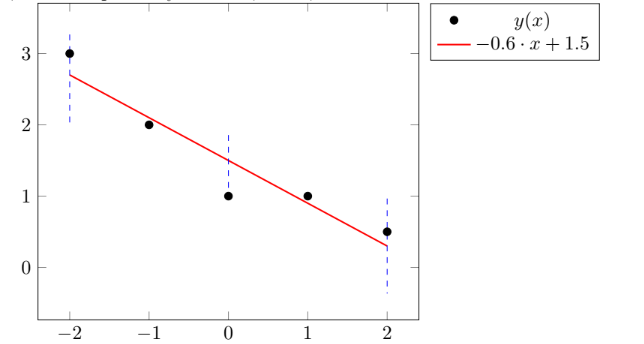
\includegraphics[width=\linewidth]{Graph.png}
	\caption{Note the interval lengths.}
	\label{fig:pairs}
\end{figure}

\begin{problem}{11.44}
\end{problem}

We have $\hat{\beta}_0 = 21.575$, $\hat{beta}_1 = 4.842$, $S_{xx} = 42$, $\bar{x} = 4.5$, and $n = 8$.\\

This gives us $s = 1.74575$.\\

When $x^* = 10$, we get
\begin{align*}
	&\hat{\beta}_0 + \hat{\beta}_1x^* \pm t_{\alpha/2}S\sqrt{1 + \frac{1}{n} + \frac{(x^* - \bar{x})^2}{S_{xx}}}\\
	= &21.575 + (4.842)(10) \pm 2.447(1.74575)\sqrt{1 + \frac{1}{8} + \frac{(10 - 4.5)^2}{42}}
\end{align*}

This yields a confidence interval of $(64.198, 75.795)$.\\

When $x^* = 11$, we get
\begin{align*}
	&\hat{\beta}_0 + \hat{\beta}_1x^* \pm t_{\alpha/2}S\sqrt{1 + \frac{1}{n} + \frac{(x^* - \bar{x})^2}{S_{xx}}}\\
	= &21.575 + (4.842)(11) \pm 2.447(1.74575)\sqrt{1 + \frac{1}{8} + \frac{(11 - 4.5)^2}{42}}
\end{align*}

This yields a confidence interval of $(68.597, 81.069)$.\\

We should not feel comfortable using this model and the data of Exercise 11.5 to predict the median sale price for the year 1988 because the width of the confidence intervals increases as you move farther away from the mean, and the data in Exercise 11.5 is very far from $\bar{x} = 4.5$.

\end{document}